\documentclass[xcolor=table]{beamer}
\usetheme[progressbar=frametitle]{metropolis}
\setbeamercolor{block body}{bg=mDarkTeal!30}
\setbeamercolor{block title}{bg=mDarkTeal,fg=black!2}
\usepackage{amsmath}
\usepackage{xcolor}
\usepackage{hyperref}
\hypersetup{
colorlinks = true,
linkcolor =.,
    citecolor = .,
    urlcolor = blue
}
\usepackage{cancel}
\usepackage{amssymb}
\usepackage{comment}
\usepackage{witharrows}
\usepackage{mathtools}
\usepackage{multicol}

\newcommand{\pstar}{p^\star(y \mid \bx)}
\newcommand{\pred}{p(y \mid \bx)}
\newcommand{\xind}{\mathcal X_{IND}}

%21-JUN-2016


% Example definitions.
% --------------------

% Specific definitions
\def\Xtr{\mathbf{X}_{\text{tr}}}
\def\Ztr{\mathbf{Z}_{\text{tr}}}

% Packages
\usepackage{bm}
\usepackage{color}
\usepackage{amssymb}

%\usepackage{cite}
%\usepackage[pdftex]{graphicx}
\usepackage{algorithm,algorithmic}
\usepackage{amsmath}
\usepackage{url}
\usepackage{float}
\usepackage{cancel}

\usepackage{multirow}

% Functions
\def\trace{\operatorname{Tr}}
\def\KL{\mathbf{KL}}
\def\PG{\operatorname{PG}}
\newcommand{\E}{\mathbb{E}}

% Number Sets
\def\R{{\mathbb R}}
\def\Z{{\mathbb Z}}
\def\N{{\mathbb N}}

% Text
\def\p{{\mathrm{p}}}
\def\q{{\mathrm{q}}}
\def\rd{{\mathrm{d}}}

\def\F{{\mathrm{F}}}
\def\G{{\mathrm{G}}}
\def\H{{\mathrm{H}}}
\def\T{{\mathrm{T}}}

\def\KL{{\mbox{KL}}}
\def\TV{{\mbox{TV}}}

\def\tr{{\text{tr}}}

% Cal
\def\cC{{\mathcal C}}
\def\cH{{\mathcal H}}
\def\cL{{\mathcal L}}
\def\cN{{\mathcal N}}
\def\cX{{\mathcal X}}

% Bold Symbols and numbers
\def\bzero{{\mathbf 0}}
\def\bone{{\mathbf 1}}

% Greek letters
\def\balpha{{\boldsymbol{\alpha}}}
\def\bbeta{{\boldsymbol{\beta}}}
\def\bgamma{{\boldsymbol{\gamma}}}
\def\bdelta{{\boldsymbol{\delta}}}
\def\bepsilon{{\boldsymbol{\epsilon}}}
\def\bheta{{\boldsymbol{\eta}}}
\def\btheta{{\boldsymbol{\theta}}}
\def\biota{{\boldsymbol{\iota}}}
\def\bkappa{{\boldsymbol{\kappa}}}
\def\blambda{{\boldsymbol{\lambda}}}
\def\bmu{{\boldsymbol{\mu}}}
\def\bnu{{\boldsymbol{\nu}}}
\def\bxi{{\boldsymbol{\xi}}}
\def\bpi{{\boldsymbol{\pi}}}
\def\brho{{\boldsymbol{\rho}}}
\def\bsigma{{\boldsymbol{\sigma}}}
\def\btau{{\boldsymbol{\tau}}}
\def\bups{{\boldsymbol{\upsilon}}}
\def\bphi{{\boldsymbol{\phi}}}
\def\bchi{{\boldsymbol{\chi}}}
\def\bpsi{{\boldsymbol{\psi}}}
\def\bomega{{\boldsymbol{\omega}}}

\def\bAlpha{{\boldsymbol{\Alpha}}}
\def\bBeta{{\boldsymbol{\Beta}}}
\def\bGamma{{\boldsymbol{\Gamma}}}
\def\bDelta{{\boldsymbol{\Delta}}}
\def\bEpsilon{{\boldsymbol{\Epsilon}}}
\def\bHeta{{\boldsymbol{\Eta}}}
\def\bTheta{{\boldsymbol{\Theta}}}
\def\bIota{{\boldsymbol{\Iota}}}
\def\bKappa{{\boldsymbol{\Kappa}}}
\def\bLambda{{\boldsymbol{\Lambda}}}
\def\bMu{{\boldsymbol{\Mu}}}
\def\bNu{{\boldsymbol{\Nu}}}
\def\bXi{{\boldsymbol{\Xi}}}
\def\bPi{{\boldsymbol{\Pi}}}
\def\bRho{{\boldsymbol{\Rho}}}
\def\bSigma{{\boldsymbol{\Sigma}}}
\def\bTau{{\boldsymbol{\Tau}}}
\def\bUps{{\boldsymbol{\Upsilon}}}
\def\bPhi{{\boldsymbol{\Phi}}}
\def\bChi{{\boldsymbol{\Chi}}}
\def\bPsi{{\boldsymbol{\Psi}}}
\def\bOmega{{\boldsymbol{\Omega}}}

% Bold
\def\ba{{\mathbf a}}
\def\bb{{\mathbf b}}
\def\bc{{\mathbf c}}
\def\bd{{\mathbf d}}
\def\be{{\mathbf e}}
\def\bff{{\mathbf f}}
\def\bg{{\mathbf g}}
\def\bh{{\mathbf h}}
\def\bi{{\mathbf i}}
\def\bj{{\mathbf j}}
\def\bk{{\mathbf k}}
\def\bl{{\mathbf l}}
\def\bm{{\mathbf m}}
\def\bn{{\mathbf n}}
\def\bo{{\mathbf o}}
\def\bp{{\mathbf p}}
\def\bq{{\mathbf q}}
\def\br{{\mathbf r}}
\def\bs{{\mathbf s}}
\def\bt{{\mathbf t}}
\def\bu{{\mathbf u}}
\def\bv{{\mathbf v}}
\def\bw{{\mathbf w}}
\def\bx{{\mathbf x}}
\def\by{{\mathbf y}}
\def\bz{{\mathbf z}}

\def\bA{{\mathbf A}}
\def\bB{{\mathbf B}}
\def\bC{{\mathbf C}}
\def\bD{{\mathbf D}}
\def\bE{{\mathbf E}}
\def\bF{{\mathbf F}}
\def\bG{{\mathbf G}}
\def\bH{{\mathbf H}}
\def\bI{{\mathbf I}}
\def\bJ{{\mathbf J}}
\def\bK{{\mathbf K}}
\def\bL{{\mathbf L}}
\def\bM{{\mathbf M}}
\def\bN{{\mathbf N}}
\def\bO{{\mathbf O}}
\def\bP{{\mathbf P}}
\def\bQ{{\mathbf Q}}
\def\bR{{\mathbf R}}
\def\bS{{\mathbf S}}
\def\bT{{\mathbf T}}
\def\bU{{\mathbf U}}
\def\bV{{\mathbf V}}
\def\bW{{\mathbf W}}
\def\bX{{\mathbf X}}
\def\bY{{\mathbf Y}}
\def\bZ{{\mathbf Z}}

% Commands
%--------------------
\newcommand{\mean}[1]{\mathrm{<}#1\mathrm{>}}


%\newcommand{\d}{{\mathrm d}}
\DeclareMathOperator*{\diag}{diag}


% Theorems

\usepackage{amsthm}
\theoremstyle{definition}

\newtheorem{proposition}[]{Proposition}
%\newtheorem{problem}[]{Problem}

\usepackage{arydshln}
\usepackage{natbib}
 


\DeclarePairedDelimiter\abs{\lvert}{\rvert}%
\DeclarePairedDelimiter\norm{\lVert}{\rVert}%

\begin{document}

\title{Simple and Principled Uncertainty Estimation with
Deterministic Deep Learning via Distance Awareness}
%\subtitle{Combining continuous-valued outputs}
\author[Javier Sáez]{\textbf {Javier Sáez}} % auteur
\institute[University of Granada]{\textbf {University of Granada}\\
Visual Information Processing Group}
\date{\today}

\begin{frame}
    \maketitle
\end{frame}

\begin{frame}{Index}
    \tableofcontents

    Paper: \citep{sngp}
\end{frame}


%%%%%%%%%%%%%%%%%%%%
%%%%%% SECTION %%%%%
%%%%%%%%%%%%%%%%%%%%

\section{Introduction}

\begin{frame}{Introduction}
    \begin{itemize}
        \item Real world applications \textbf{need} efficient methods that reliably quantify a deep neural network's (DNN) predictive uncertainty.

        \pause

        \item Examples: 
        \begin{itemize}
            \item Object detection in autonomous driving
            \item Ad click prediction in websites
            \item Understanding in a conversational system (ChatGPT)
            \item Domain-specific chatbot services (weather)
        \end{itemize}

        
    \end{itemize}
\end{frame}

\begin{frame}{Introduction}

    \begin{itemize}
        \item \textbf{Problem:} The performance of the models can be arbitrarily bad when the new input is far from the training set.
        
        \pause

        \item \textbf{Need:} Methods that return a uniform distribution (max entropy) over output labels if the input is far. 
    \end{itemize}
    \pause \textbf{GPs!}\\
    
GPs need a previous feature extraction. We would like the DNN to be \emph{distance aware}.
\end{frame}

%%%%%%%%%%%%%%%%%%%%
%%%%%% SECTION %%%%%
%%%%%%%%%%%%%%%%%%%%

    
\begin{frame}{Notation}
\begin{itemize}
\item Consider the data distribution \(\pstar\), where \(y \in \{1,\dots,K\}\) and \(x \in \mathcal X \subset \R^d\), where \(\mathcal X\) is the data manifold with a suitable metric \(\norm{\cdot}_{X}\).
\pause
\item In practise, data is collected from a subset \(\xind \subset \mathcal X\). As a result,
\begin{align*}
\pstar & = p^\star(y, \bx \in \xind \mid \bx) + p^\star(y, \bx \notin \xind \mid \bx)\\ 
& = p^\star(y \mid \bx , \bx \in \xind) \cdot p^\star( \bx \in \xind \mid \bx) \\
& \quad+ p^\star(y \mid \bx , \bx \notin \xind) \cdot p^\star( \bx \notin \xind \mid \bx)
\end{align*}
Models learn \(p^\star(y \mid \bx, \bx \in \xind)\). \\
However, \(p^\star(y \mid \bx, \bx \notin \xind)\) can be very different.
\pause
\item In testing, models use a predictive \(p(y \mid \bx)\) for any \(\bx \in \mathcal X = \xind \cup \mathcal X_{OOD}\). \(\mathcal X_{OOD}\) can be very different even in a certain topic (user asking for earthquakes in a weather-themed chatbot)!
\end{itemize}

\vspace{1cm}

\end{frame}

\subsection{Uncertainty estimation as Minimax Learning Problem}

\begin{frame}{Towards the loss function}

If the model predicts class \(y\) with confidence \(\hat p\), we would like the model to be correct \(\hat p\) of the times. In that case, the model is said to be \textbf{callibrated}. Formally, the model is calibrated if
\[
\mathbb P(\hat y = y_{true} \mid \hat p = p ) = p
\]

%Suppose a model predicts a class \(y\) with probability \(\hat p\). The model is \textbf{calibrated} if \(\hat p = p\), where \(p\) is the true probability. Formally:
%\[
%\mathbb P(Y = y\mid \hat p = p) = p.
%\]
We can take the expectation in the possible predicted confidences \(\hat p\), leading to the Expected Calibration Error (ECE) \citep{ECE2017}:
\[
ECE = \mathbb E_{\hat p}  \left[ \abs{ \mathbb \mathbb P(\hat y = y_{true} \mid \hat p = p ) - p}\right]
\]
However, this loss function is not suitable for this case, since it is not uniquely minimized.\\




\end{frame}

\begin{frame}{Towards the loss function}
    \begin{definition}
A scoring rule\footnote{\href{https://en.wikipedia.org/wiki/Scoring_rule}{Wikipedia's link}} is any extended real-valued function \({\displaystyle \mathbf {S} :{\mathcal {P}}\times \Omega \rightarrow \mathbb {R} }\) such that \( {\displaystyle \mathbf {S} (P,\cdot )}\) is \({\mathcal {P}}\)-quasi-integrable for all \( P\in {\mathcal {P}}\).
\end{definition}
 \( {\displaystyle \mathbf {S} (P,y)}\) represents the loss or penalty when the prediction  \(P\in {\mathcal {P}} \) is issued and the observation \(y\in \Omega\) materializes. 
\end{frame}


\begin{frame}{Example: Brier's Score}
    An example of a strictly proper scoring rule is the \textbf{Brier's score}, defined as:
    \[
    B(p,y) = \sum_{j=1}^C (y_j - p_j)^2  ,
    \]
    where 
    \begin{itemize}
        \item \(y_j = 1\) if the the input belongs to class \(j\)-th and \(0\) otherwise, 
        \item \(C\) is the number of classes and
        \item \(p_j\) is the probability assigned to class \(j\).
    \end{itemize}
    
\end{frame}

\begin{frame}{Towards the loss function}
If the label \(y\) is sampled from a distribution \(Q\), the expected score under \(Q \in \mathcal P\) can be written as:
\[
\mathbf S (P,Q) = \int \mathbf s (P,y)\ d Q(y).
\]
\pause
We can define a \textbf{divergence} of \(P\) from \(Q\) as:
\[
d(P,Q) \triangleq \mathbf{S}(P,Q) - \mathbf{S}(Q,Q).
\]
    
\end{frame}

\begin{frame}{Towards the loss function}
    \begin{definition}
        A scoring rule \(\mathbf S\) is proper \emph{relative to} \(\mathcal P\) if
        \[
        d(P,Q ) \geq 0, \quad \forall P,Q \in \mathcal P.
        \]
    \end{definition}
    Also, it is \textbf{strictly proper} \citep{2007:SPR} if the above equation holds with equality if, and only if, \(P = Q\).
\end{frame}


\begin{frame}{Towards the loss function}
    Consider the vector of calibrated probabilities \(\bC = (C_1,\dots,C_k)\) and let \(P\) be the output probabilities of a model. Using \(\bC\),  the expected loss according a P.S.R. can be expressed \citep{kull2015novel} as:
    \[
    \mathbb{E}\left[d(P,Y)\right] = \mathbb{E}[d(P,\bC)] + \mathbb E [ d(\bC,Y)]
    \]

    \textbf{Consequence:} Each PSR is an upper bound of the calibration error, so minimizing a PSR implies minimizing the calibration error.
\end{frame}


\begin{frame}{Towards the loss function}
    
    The problem of uncertainty quantification turns into constructing an optimal \(p\) to minimize the expected risk over \(\mathcal X\):
    \begin{align}
    \inf_{p \in \mathcal P} S(p, p^*) = 
    \inf_{p \in \mathcal P} \underset{\bx \in \mathcal X}{\mathbb E}
    \left[s(p, p^*|\bx) \right].
    \label{eq:brier_risk}
    \end{align}
    \pause
    However, this is not possible to solve since data only comes from \(\mathcal X_{IND}\), OOD distribution is never learned, so generalization is not guaranteed. We then take a \emph{Minimax} strategy (minimize the worst-case risk):
    \pause
    \begin{align}
\inf_{p \in \mathcal P} \left[ \sup_{p^* \in \mathcal P^*} \; S(p, p^*) \right].
\label{eq:minimax_loss}
\end{align}
\end{frame}

\begin{frame}{Solution using Brier's Score}
    Under the classification task and using Brier's score, the solution to Eq. \eqref{eq:minimax_loss} is:
    \begin{align*}
    p(y |\bx) 
    &= 
    p(y|\bx, \bx \in \xind) * p^*(\bx \in \xind \mid \bx) \\
    &  \quad+ 
    p_{\textup{\texttt{uniform}}}(y|\bx, \bx \notin \xind) * p^*(\bx \not\in \xind \mid \bx).
    \label{eq:minimax_solution}
\end{align*}

Advantages:
\begin{itemize}
    \item Intuitive!
    \item Verifies that there is the unique optimal solution to the problem in Eq. \eqref{eq:minimax_loss}
\end{itemize}
Disadvantage:
\begin{itemize}
\item We have to assume that the model can quantify \(p^\star (\bx \in \xind \mid \bx)\) well.
\end{itemize}

\end{frame}
%%%%%%%%%%%%%%%%%%%%
%%%%%% SECTION %%%%%
%%%%%%%%%%%%%%%%%%%%

\subsection{Input Distance Awareness}

\begin{frame}{Input Distance Awareness}
    We need a notion of distance between a new example and \(\xind\)!
    \pause

    \begin{definition}[Input Distance Awareness]
        Consider a predictive distribution \(p(y \mid \bx)\) trained on \(\xind\). We say that it is \textbf{input distance aware} if:\\
        
            Exists \(u(\bx)\) a summary statistic of \(\pred\) such that:
        \begin{enumerate}
            \item quantifies model uncertainty (eg: predictive variance) and
            \item reflects the distance between \(\bx\) and training data w.r.t. \(\norm{\cdot}_{\mathcal X}\)
        \end{enumerate}
        \[
        u(\bx) = v(d(\bx, \xind)),
        \]
        where \(v\) is a monotonic function and 
        \[d(\bx,\xind) = \mathbb E_{x' \sim \xind} \norm{\bx -\bx'}^2_{X}
        \]
    \end{definition}
\end{frame}


\begin{frame}{Example: Gaussian Processes}



GPs with RBF kernel are input distance aware models:
\begin{itemize}
    \item Predictive \(\pred = softmax(g(\bx))\)
    \item Exists \(u(\bx^\star) = var(g(\bx^\star)) = 1- \bk^{\star^T} \bV \bk^\star\), with
    \[
    \bk_i^\star = \exp \left( -\gamma \norm{\bx^\star - \bx_i}_{X}^2\right)
    \]
\end{itemize}
\pause
In a typical DL model, the confidence in a class is computed in a dense layer as:
\[
\text{logit}_k(\bx) = h(\bx)^\top \beta_k.
\]
The model decission is not based on its distance to training data \(\xind\), but on its distance to the decission boundaries.
    
\end{frame}

\begin{frame}{Conditions for IDA in Deep Learning}
Consider a DL model \(logit(\bx) = g \circ h(\bx)\) where 

\begin{itemize}
    \item \(h\) creates a representation of \(\bx\) and
    \item \(g\) maps \(h(\bx)\) to the label space. 
\end{itemize} 
To make this model distance aware we need:
\pause
\begin{enumerate}
    \item Make the output layer \(g\) distance aware, so it outputs an uncertainty metric reflecting distance in the representation space
    \pause
    \item Make the hidden mapping \(h\) \emph{distance preserving}. 
    \pause 
    Mathematically, that is fullfilling the bi-Lipschitz condition:
    \[
    \underbrace{L_1 \ \norm{\bx_1-\bx_2}_X}_{\text{not unnecessarily invariant}} \leq \norm{h(\bx_1) - h(\bx_2)}_H \leq \underbrace{L_2 \ \norm{\bx_1 - \bx_2}_X}_{\text{robustness}},
    \]
    where \(0 < L_1 < 1 < L_2\). This condition encourages \(h\) to be approximately isometric.
\end{enumerate}
    
\end{frame}
%%%%%%%%%%%%%%%%%%%%
%%%%%% SECTION %%%%%
%%%%%%%%%%%%%%%%%%%%

\section{SNGP: Spectral-normalized Neural Gaussian Process}

\begin{frame}{Visual description}
\begin{figure}
    \centering
    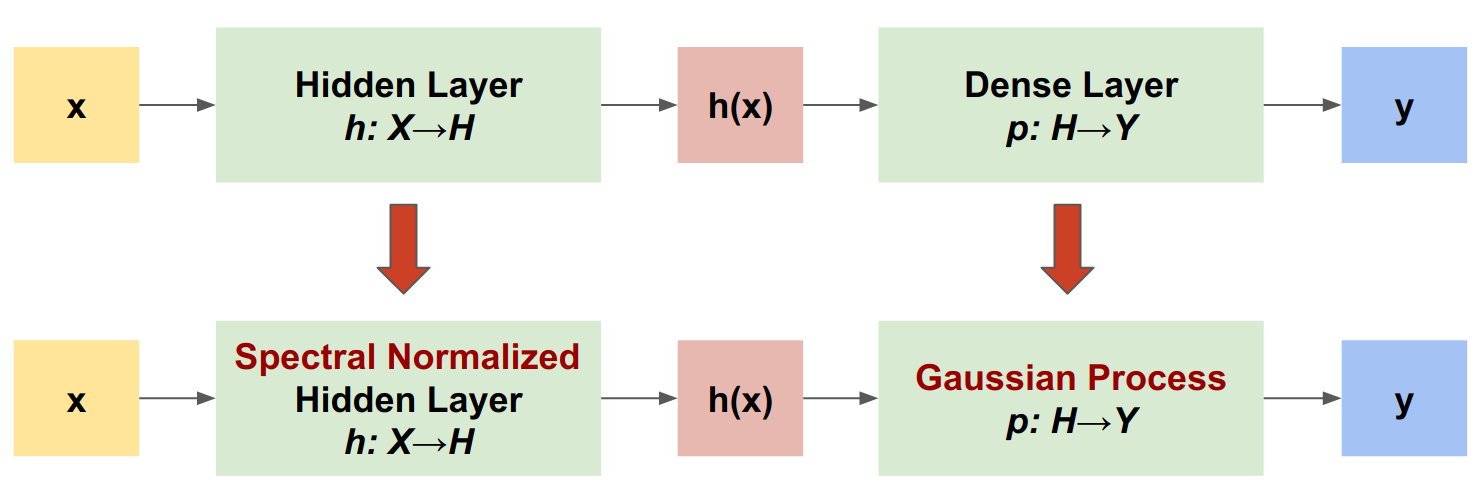
\includegraphics[scale=0.2]{fig/sngp.png}
    \caption{Visual description from the provided \href{https://colab.research.google.com/github/tensorflow/docs/blob/master/site/en/tutorials/understanding/sngp.ipynb}{tutorial}.}
    \label{fig:description}
\end{figure}
    
\end{frame}

\subsection{Distance-aware Output Layer via Laplace-approximated Neural Gaussian Process}

\begin{frame}{Distance-aware Output Layer}
To make the output layer \(g\) distance aware, the model replaces the typical dense layer with a \textbf{GP with RBF Kernel}. \\
\vspace{1cm}
Specifically, given \(\{\bx_i,y_i\}_{i=1}^N\), we place the usual prior to the output layer \(g_{N \times 1}=[g(h_1),\dots,g(h_N)]^T\):
\[
g_{N \times 1} \sim GP(\mathbf{0}, \bK_{NN}), \quad \bK_{i,j} = \exp(-\norm{h_i-h_j}_2^2/2).
\]
\\
\pause
As per usual with GPs, computing the exact posterior distribution is intractable.
    
\end{frame}

\begin{frame}{Distance-aware Output Layer: Approximating GP Prior}

The GP prior is approximated using \textbf{Random Fourier Features} (RFF)
\[
    \bg_{N \times 1} \sim GP(\bzero, \bPhi\bPhi^\top), 
     \qquad 
    \bPhi_{i, D_L \times 1} = 
    \sqrt{2/D_L} * 
    \cos(-\bW_L h_i + \bb_L),
    \label{eq:rff_gp}
\]
where \(w_{ij} \sim \mathcal N(0,1)\) and \(b_k \sim Uniform(0,2\pi)\).\\
\pause
As a result, for the \(k^{th}\) logit, this approximation can be written as a NN layer:
\[
    g_k(h_i) = \sqrt{2/D_L} * \cos(-\bW_L h_i + \bb_L)^\top \bbeta_k, 
\]
where \(\bW\) is fixed and the prior of \(\mathbf \beta_k\) is\(\bbeta^k_{D_L \times 1} \sim \mathcal N(0, \mathbf I_{D_L \times D_L})\).\\
\end{frame}


\begin{frame}{Distance-aware Output Layer: Posterior Approximation}
    
\textbf{Consequence:} We have reduced the infinite-dimensional GP to a Bayesian linear model, so we can apply one of the known posterior approximation methods.
\vspace{0.3cm}
\pause
\begin{definition}[Laplace approximation]
    Laplace method approximates the posterior distribution \(p(\beta \mid \mathcal D)\) using a Gaussian distribution centered at the MAP estimate \(\hat \beta = \text{arg}\max_\beta p(\beta \mid \mathcal D)\) and covariance matrix the inverse of the Hessian of the log posterior likelihood evaluated at \(\hat \beta\), that is:
    \[
    p(\beta_k \mid \mathcal D) \approx \mathcal N(\hat \beta_k, \hat \bH_k^{-1}),
    \]
    with \( \hat{\bH}_{k, (i,j)} = \frac{\partial^2}{\partial \beta_i \partial \beta_j} \log \, p(\beta_k|\mathcal D)|_{\beta_k=\hat{\beta}_k}\)
\end{definition}
\end{frame}

\begin{frame}{Distance-aware Output Layer: Results}
The GP posterior can be learned:
    \begin{itemize}
        \item scalably,
        \item in closed form,
        \item with minimal modification to the training of a deterministic DNN,
        \item by the Bernstein-von-Mises theorem \citep{BvMth}, the Laplace approximation ot the RFF posterior is asymptotically exact.
    \end{itemize}
\end{frame}

\subsection{Distance-preserving Hidden Mapping via Spectral Normalization}

\begin{frame}{Distance-preserving Hidden Mapping}
The last goal is to ensure that the hidden mapping \(h\) is \emph{distance preserving} so that the distance in the hidden space \(\norm{h(\bx) - h(\bx')}_H\) has a meaningful correspondence to the distance in the input space \(\norm{\bx - \bx'}_X\).\\
\pause
\begin{nnote}[Assumption]
The used models will be residual DL models (ResNets, Transformers), composed of residual blocks 
\begin{equation}\label{eq:residual:arch}
h(\bx) = h_{L-1} \circ \cdots \circ h_1(\bx), \quad h_l(\bx) = \bx + f_l(\bx).
\end{equation}
\end{nnote}

\end{frame}

\begin{frame}{Distance-preserving Hidden Mapping}
    \begin{proposition}
    Let \(h: \mathcal X \to \mathcal H\) be a hidden mapping with residual architecture \eqref{eq:residual:arch}. If for \(0 < \alpha \leq 1\), all \(f_l\) are \(\alpha-\)Lipschitz, that is: 
    \[
    \norm{f_l(\bx) - f_l(\bx')}_H \leq \alpha \norm{\bx - \bx'}_X\text{ for all } (\bx,\bx') \in \mathcal X,
    \]
    then:
    \[
    L_1 \cdot \norm{\bx - \bx'}_X \leq \norm{h(\bx) - h(\bx')}_H \leq L_2 \cdot \norm{\bx - \bx'}_X,
    \]
    where \(L_1 = (1-\alpha)^{L-1}\) and \(L_2 = (1+\alpha)^{L-1}\).
    \end{proposition}
    This result implies that if the previous conditions are fulfilled, \(h\) is distance preserving.
\end{frame}

\begin{frame}{Distance-preserving Hidden Mapping}
If \(f_l(\bx) = \sigma(\bW_l \bx + \bb_l)\) is the residual block, since
\[
\norm{f_l}_{Lip} \leq \norm{\bW_l \bx + \bb_l}_{Lip} \leq \norm{\bW_l}_2,
\]
it is sufficient to have \(\norm{\bW_l}_2 \leq 1\) to ensure \(h\) is distance preserving.
\pause
\begin{definition}[Spectral Normalization]
    Let \(\lambda = \norm{\bW_l}_2\) be the spectral norm of \(\bW_l\). Then, the spectral normalization is performed as:
\begin{equation}\label{eq:spectral:normal}
    \bW_l = \begin{cases} c \cdot \bW_l / \lambda & \text{ if } c < \lambda \\
    \bW_l & \text{ otherwise}
    \end{cases}
\end{equation}
where \(c > 0\) is a hyperparameter used as a threshold.
\end{definition}

The hyperparameter is useful since it helps with the regularization of the model.

\end{frame}

\begin{frame}{Method summary: Prediction}


\begin{algorithm}[H]
   \caption{SNGP Prediction}
   \label{alg:prediction}
\begin{algorithmic}[1]
   \STATE {\bfseries Input:} Testing example $\bx$.
%   \STATE {\bfseries Prediction:} \\
   \STATE %$\bullet$ 
   Compute Feature: %$\bPhi_{D_L \times 1} = \sqrt{2/D_L} * \cos(\bW_L h(\bx) + \bb_L).$
   \vspace{-0.5em}
   $$\bPhi_{D_L \times 1} = \sqrt{2/D_L} * \cos(\bW_L h(\bx) + \bb_L),$$ 
   \vspace{-1.2em}
   \STATE %$\bullet$ 
   Compute Posterior Mean: %Prediction: 
   %$logit_k(\bx)=\Phi^\top\bbeta_k.$ %\\
   \vspace{-0.5em}
   $$\text{logit}_k(\bx)=\Phi^\top\bbeta_k$$ 
   \vspace{-1.2em}
   \STATE %$\bullet$ 
   Compute Posterior Variance: %Uncertainty: %$\var_k(\bx)=\Phi^\top\hat{\Sigma}_k\Phi.$
   %\\
   \vspace{-0.5em}
   $$\text{var}_k(\bx)=\Phi^\top\hat{\Sigma}_k\Phi.$$ 
   \vspace{-1em}
      \STATE %$\bullet$ 
      Compute Predictive Distribution:\\
   \vspace{-1.5em}
   $$p(y|\bx)=\int_{m \sim N(\text{logit}(\bx), \text{var}(\bx))}{\text{softmax}(m)}$$ 
   \vspace{-1em}
   %\STATE $\;\;$ for $m \sim N(\text{logit}(\bx), var(\bx)).$
%   \STATE $\bullet$ Compute Predictive Distribution:\\
%   \vspace{-0.5em}
%   $$p(\bx)=\mathsf{softmax}(m)$$ 
%   \vspace{-1em}
%   \STATE $\;\;$ for $m \sim N(logit(\bx), var(\bx)).$
   %\balaji{add Monte Carlo sampling for completeness?}
   %\balaji{slightly different from definition in $u(\bx^*)=var(g(\bx^*)) = 1 - \bk^{*\top}\bV\bk^*$}
  % \vspace{-1em} 
\end{algorithmic}
\end{algorithm}

\end{frame}

\begin{frame}{Results}
    \begin{figure}
        \centering
        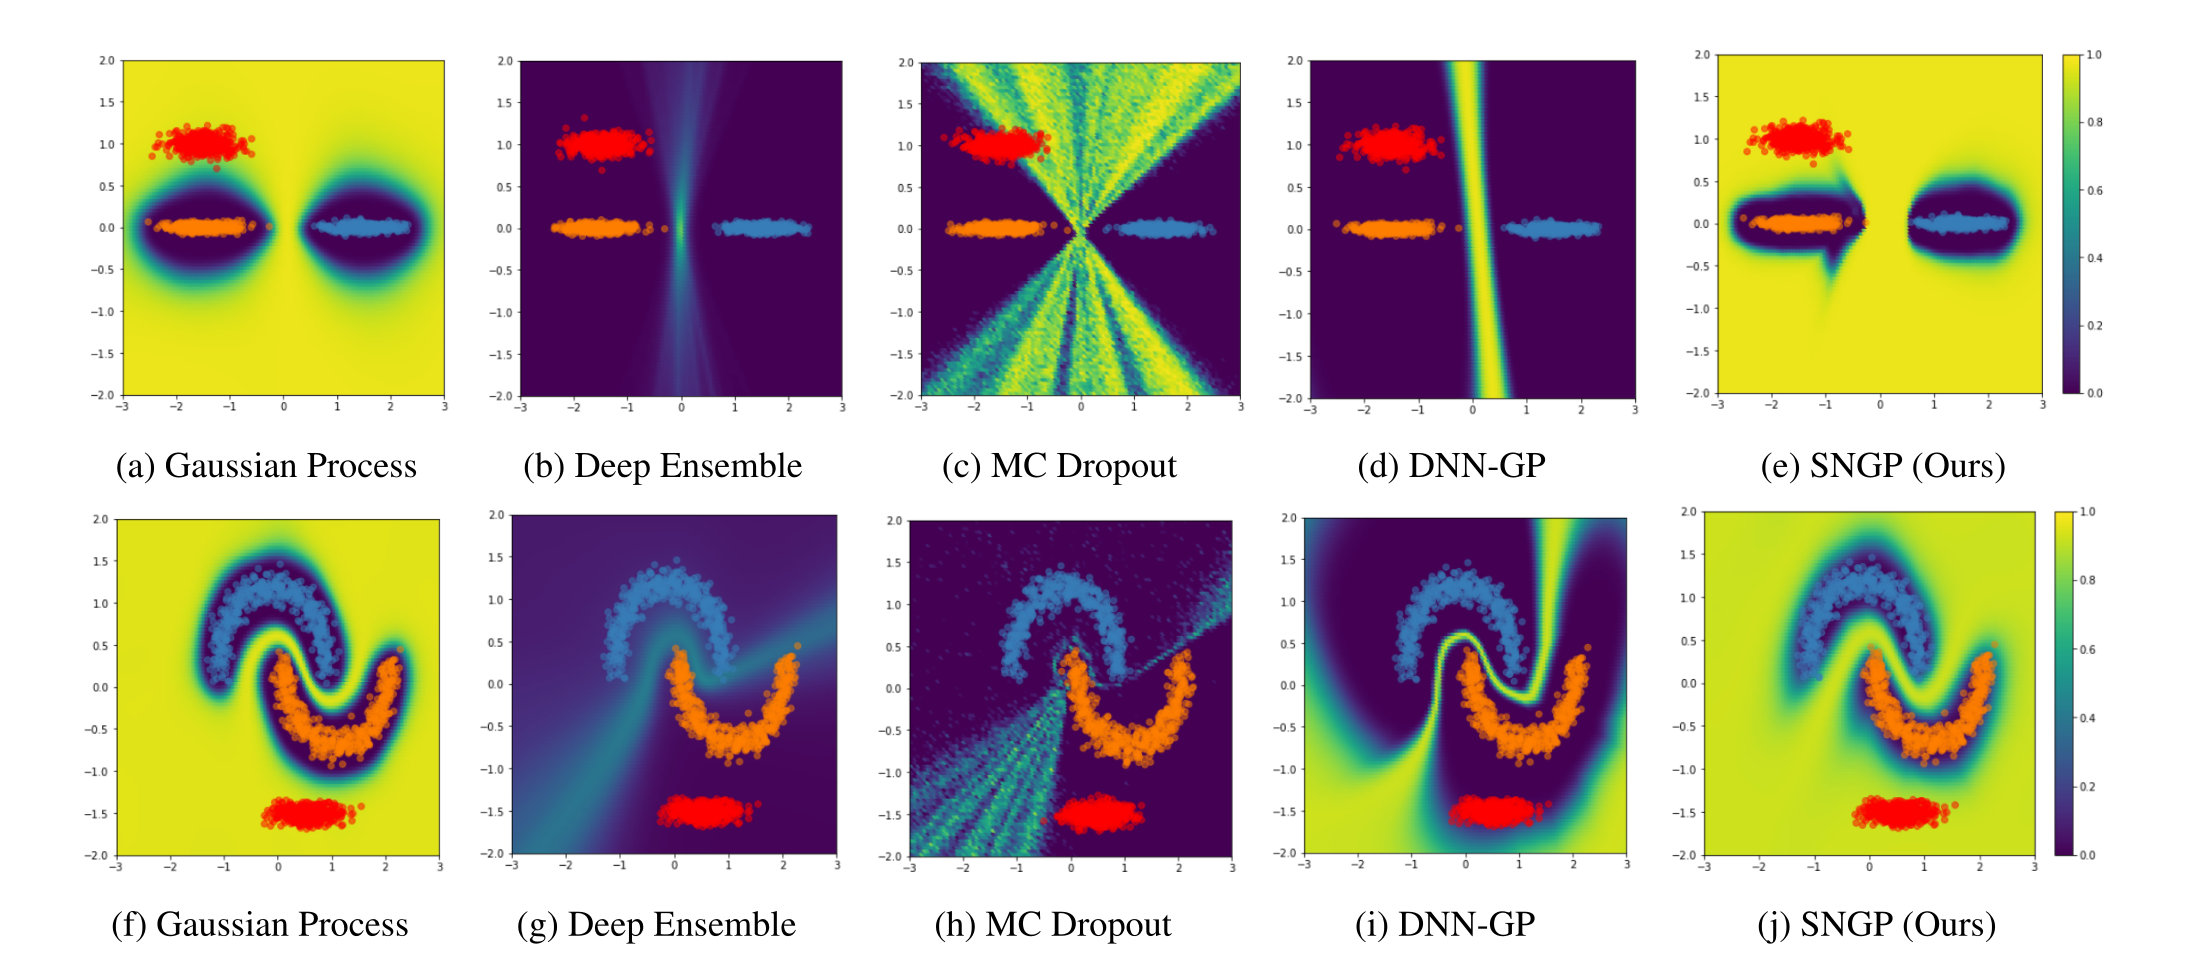
\includegraphics[scale=0.15]{fig/SNGP_results.png}
        \label{fig:results}
    \end{figure}
\end{frame}

\begin{frame}{Results: OOD metrics}

To evaluate the model performance in OOD detection in this task, the \textbf{model's uncertainty estimate} is used as a predictive score for OOD classification. 

\begin{equation} \label{eq:DSU}
u(\bx) = \frac{K}{K + \sum_{i=1}^K \exp(\text{logit}_i(h(\bx))}.
\end{equation}

    
\end{frame}


\begin{frame}{Results: OOD Evaluation}
    \begin{enumerate}
    \item Generate the dataset \href{https://github.com/google/uncertainty-baselines/blob/9cef4b58b8b8bc9b3b3478ed364e30fd7bbe5a25/uncertainty_baselines/datasets/base.py}{adequately}: merge two datasets (in-distribution and OOD) in one and add a new label (in/out distribution) to each item.
    \item Compute the logits given by the linear model representing the GP.
    \item Then, using this logits, we compute an uncertainty metric \(u(\bx)\) for each datapoint as in Equation \eqref{eq:DSU}.
    \item Create a \textbf{new binary classification problem}:  OOD class as the positive class (label \(1\)), and we take \(u(\bx)\) to be the \emph{model's} probability of this class.
    \item We compute the metrics using this probabilities and the created labels.
\end{enumerate}
\end{frame}

%%%%%%%%%%%%%%%%%%%%
%%%%%% SECTION %%%%%
%%%%%%%%%%%%%%%%%%%%





  \begin{frame}[noframenumbering]

  %\vspace{0.5cm}
  {\tiny
  \bibliographystyle{unsrtnat}
  \bibliography{bibliography.bib}
  }

  \end{frame}

  \section*{Extra slides}

  
      \begin{frame}{Definition of quasi-integrable}
    Consider
    \begin{itemize}
    \item a sample space \(\Omega\),
    \item a \(\sigma\)-algebra \( {\mathcal {A}}\) of subsets of \(\Omega\) and 
    \item a convex class \({\mathcal {F}}\) of probability measures on  \({\displaystyle (\Omega ,{\mathcal {A}})}\).
    \end{itemize}

    \begin{definition}
        
     A function defined on \(\Omega\) and taking values in the extended real line, \({\displaystyle {\overline {\mathbb {R} }}=[-\infty ,\infty ]}\), is \({\mathcal {F}}\)-quasi-integrable if it is measurable with respect to \({\mathcal {A}}\) and is quasi-integrable with respect to all \(F\in {\mathcal {F}}\). 
    \end{definition}
\end{frame}


\begin{frame}{Method summary: Training}

\begin{algorithm}[H]
   \caption{SNGP Training}
   \label{alg:training}
\begin{algorithmic}[1]
   \STATE {\bfseries Input:} \\
   Minibatches $\{D_i\}_{i=1}^N$ for $D_i=\{y_m, \bx_m\}_{m=1}^M$. %\balaji{technically, this should be inside the training loop}
   \vspace{0.2em}
   \STATE {\bfseries Initialize:} \\
  % $\hat{\bSigma}=\bI$, $\bW_L \stackrel{iid}{\sim} N(0, 1)$, $\bb_L \stackrel{iid}{\sim} U(0, 2\pi)$.\\
    \vspace{-1.2em}
    $$\hat{\bSigma}=\bI, \bW_L \stackrel{iid}{\sim} N(0, 1), \bb_L \stackrel{iid}{\sim} U(0, 2\pi)$$.\\
     \vspace{-1.2em}
%   \STATE {\bfseries Train:} \\
   \FOR{$\mathsf{train\_step}=1$ {\bfseries to} $\mathsf{max\_step}$}
   \STATE %$\bullet$ 
   SGD update $\Big\{ \bbeta, \{\bW_l\}_{l=1}^{L-1}, \{\bb_l\}_{l=1}^{L-1} \Big\}$
   \STATE %$\bullet$ 
   Spectral Normalization $\{\bW_l\}_{l=1}^{L-1}$ %as in
   (\ref{eq:spectral:normal}).
   \IF{$\mathsf{final\_epoch}$}
   \STATE %$\bullet$ 
   Update precision matrix $\{\hat{\bSigma}_{k}^{-1}\}_{k=1}^K$ % using
   (\ref{eq:precission:matrix}).
   \ENDIF
   \ENDFOR
   \STATE Compute posterior covariance $\hat{\bSigma}_k=inv(\hat{\bSigma}_k^{-1})$.
\end{algorithmic}
\end{algorithm}

\end{frame}




\begin{frame}{Implementation: Posterior precision matrix}

Under the linear-model formulation of the RFF posterior, the precision matrix has the following expression:
\begin{equation}\label{eq:precission:matrix}
\hat \Sigma_k^{-1} = \bI + \sum_{i=1}^N \hat p_{i,k}(1- \hat p_{i,k}) \Phi_i \Phi_i^T,
\end{equation}
where \(\hat p_{i,k}\) is the model prediction \(softmax(\hat g_i)\) under the MAP estimates \(\hat \beta\).\\
\pause
When using minibatches of size M, the posterior mean \(\hat \beta\) is updating via SGD with respect to the log posterior \(-\log p(\beta \mid \mathcal D)\) and the posterior precision matrix is \emph{cheaply} updated as
\[
\hat{\bSigma}^{-1}_{k,t}=(1-m)*\hat{\bSigma}^{-1}_{k, t-1} + m*\sum_{i=1}^M \hat{p}_{i,k}(1-\hat{p}_{i,k})\Phi_i \Phi_i^\top,
\]
where \(m\) is a small scaling coefficient. This computation is only performed \textbf{once at the final epoch}.



\end{frame}



\begin{frame}{Implementation: Spectral Normalization}

The spectral norm is approximated by using the \textbf{power iteration} method.
    
\end{frame}

\begin{frame}{}
    \begin{center}
        Thank you for your attention
    \end{center}
\end{frame}
\end{document}